\documentclass[]{article}
\usepackage{amsmath}
\usepackage{graphicx}
\usepackage[outdir=./]{epstopdf}
\begin{document}

\section{Principal component sharing}
%\maketitle

Tripp (2015) approximated population outputs by combining surrogate models of time-averaged output $\hat{\mathbf{f}}(\mathbf{x})$ and spike-related fluctuations $\mathbf{n}(t)$. 

In the present study we use the same noise term, but we model the static output differently. Specifically, we approximate the output as a weighted sum of principal components $\mathbf{p}_k(\mathbf{x})$ of the population's tuning curves, i.e.
\begin{equation}
\hat{\mathbf{f}}(\mathbf{x}) =  \sum_{k=1}^m \phi_k \mathbf{p}_k(\mathbf{x})
\end{equation}
where $m$ is the number of principal components used in the approximation. 

Whereas Tripp (2015) used interpolation to model each population output $\hat{\mathbf{f}}(\mathbf{x})$, here we use interpolation to model $\mathbf{p}_k(\mathbf{x})$, and then combine these linearly into approximations of the population outputs. This converges to the same result when many principal components are used, but it  
decouples the number of interpolations from the number of outputs. This is an advantage when a population has more distinct outputs than useful principal components. 

The principal components of different populations that are drawn from the same parameters are typically quite similar, as illustrated in Figure \ref{fig:pc3}. The components are usually moderately consistent between smaller populations (left panel of Figure \ref{fig:pc3}) and quite consistent between large populations (right panel of Figure \ref{fig:pc3}). In light of this consistency, we do not use the unique principal components of each individual population, but instead we use ``shared" principal components that approximate those of all the populations in a population unit. This reduces the required number of interpolation tables by up to three orders of magnitude, and allows us to leave the interpolation tables in on-chip memory throughout a simulation. To simulate each distinct population in a population unit, we need only load the unique mixing weights $\phi$ for that population (in addition to the noise parameters). This efficiency at the population-unit level is our main motivation for interpolating principal components instead of outputs. 

It turns out that principal components of different populations can also be quite similar, even if there are substantial differences in population parameters. This is illustrated in Figure \ref{fig:pc-examples}. For this reason we do not require that all populations in a population unit have exactly the same parameters. Instead, we cluster populations according to principal component similarity and assign each cluster to a population unit.   

To find mixing weights $\phi_k$ for the principal components, we first find unregularized optimal decoders $d_i^k$ for the $i^{th}$ neuron and the $k^{th}$ principal component. This allows us to estimate the variance of the noise associated with the $k^{th}$ principal component as $\sigma_k^2 = \sum_i (d_i^k)^2 \sigma^2$, where $\sigma^2$ is the noise variance of each neuron (we typically assume this to be uniform). Finally, we find regularized optimal decoders of the principal components by choosing $\phi_k$ to minimize
\begin{equation}
\int_{\mathbf{x}} d\mathbf{x} \left( \hat{\mathbf{f}}(\mathbf{x}) -  \sum_{k=1}^m \phi_k \mathbf{p}_k(\mathbf{x}) \right)^2 + \sum_{k=1}^m \phi_k \sigma_k^2
\end{equation} 

To share principal components across a population unit, we use the same $\sigma_k^2$, and simply replace the population principal components with the shared principal components. 

\begin{figure}
\centering{}
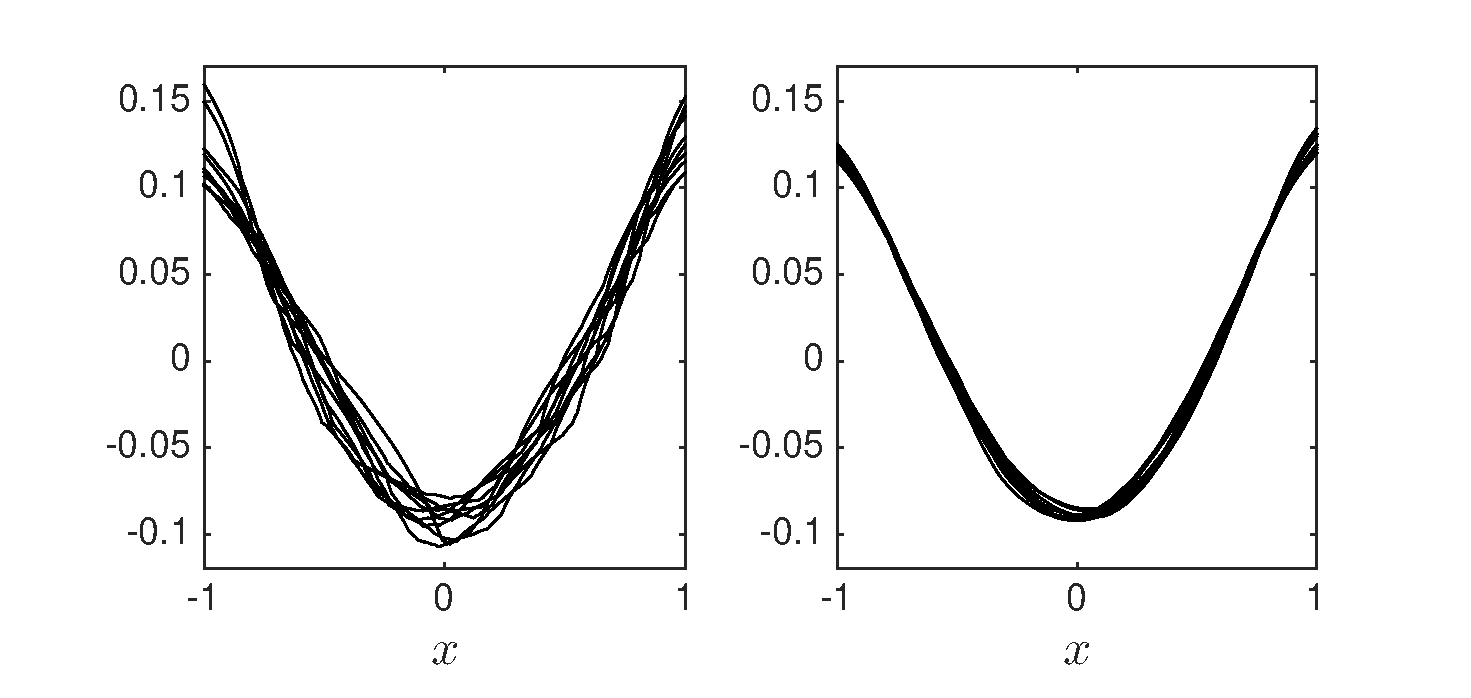
\includegraphics[scale=0.4]{PC3.eps}
\caption{The third principal components of tuning curves of random populations drawn from the same parameter distribution (parameter set \#6). The left panel shows the third principal components of ten random draws of 50 neurons. The right shows the third principal components of ten random draws of 1000 neurons. The principal components are similar in each case, and very similar across the large populations. The third principal component is shown as an example; other components have similar behaviour.}
\label{fig:pc3}
\end{figure}

\begin{figure}
\centering{}
\includegraphics[scale=0.4]{PC-examples.eps}
\caption{Tuning curves of four different example populations and their principal components. Each column corresponds to a population with different parameters (parameter sets 1, 6, 7, and 10). The top panels are 50 tuning curves drawn from populations of 1000 neurons. The bottom panels are the first six principal components of each population's tuning curves. Despite differences in parameters between the three leftmost populations, their principal components are nearly the same or nearly opposite. (To facilitate comparison across populations, the negatives of some principal components are plotted where these are more similar to corresponding components in the leftmost column.) As a counter-example, the population on the right has a very different distribution of intercepts, and very different principal components as well. }
\label{fig:pc-examples}
\end{figure}

Figure \ref{fig:shared-pcs} shows examples of static error associated with these various approximation schemes. The solid dark traces are static errors in function approximation directly from neuron tuning curves. The (fairly similar) solid light lines are static errors in function approximation from principal components of the same population. 

The dashed lines are approximation from principal components of other populations, to illustrate the potential loss in simulation accuracy associated with using shared principal components. The darker dashed line is from principal components of a larger population with the same parameters, and the lighter dashed line is from principal components of a population of the same size but different parameters. Both of these differences result in quite different static error functions than the decoding directly from tuning curves. Importantly, the error still has approximately the right frequency content, and the magnitude varies appropriately depending on the decoded function (left vs. right panels). However, the differences illustrate the importance of clustering populations so that shared principal components are as similar as possible to each population's individual principal components.   

\begin{figure}
\centering{}
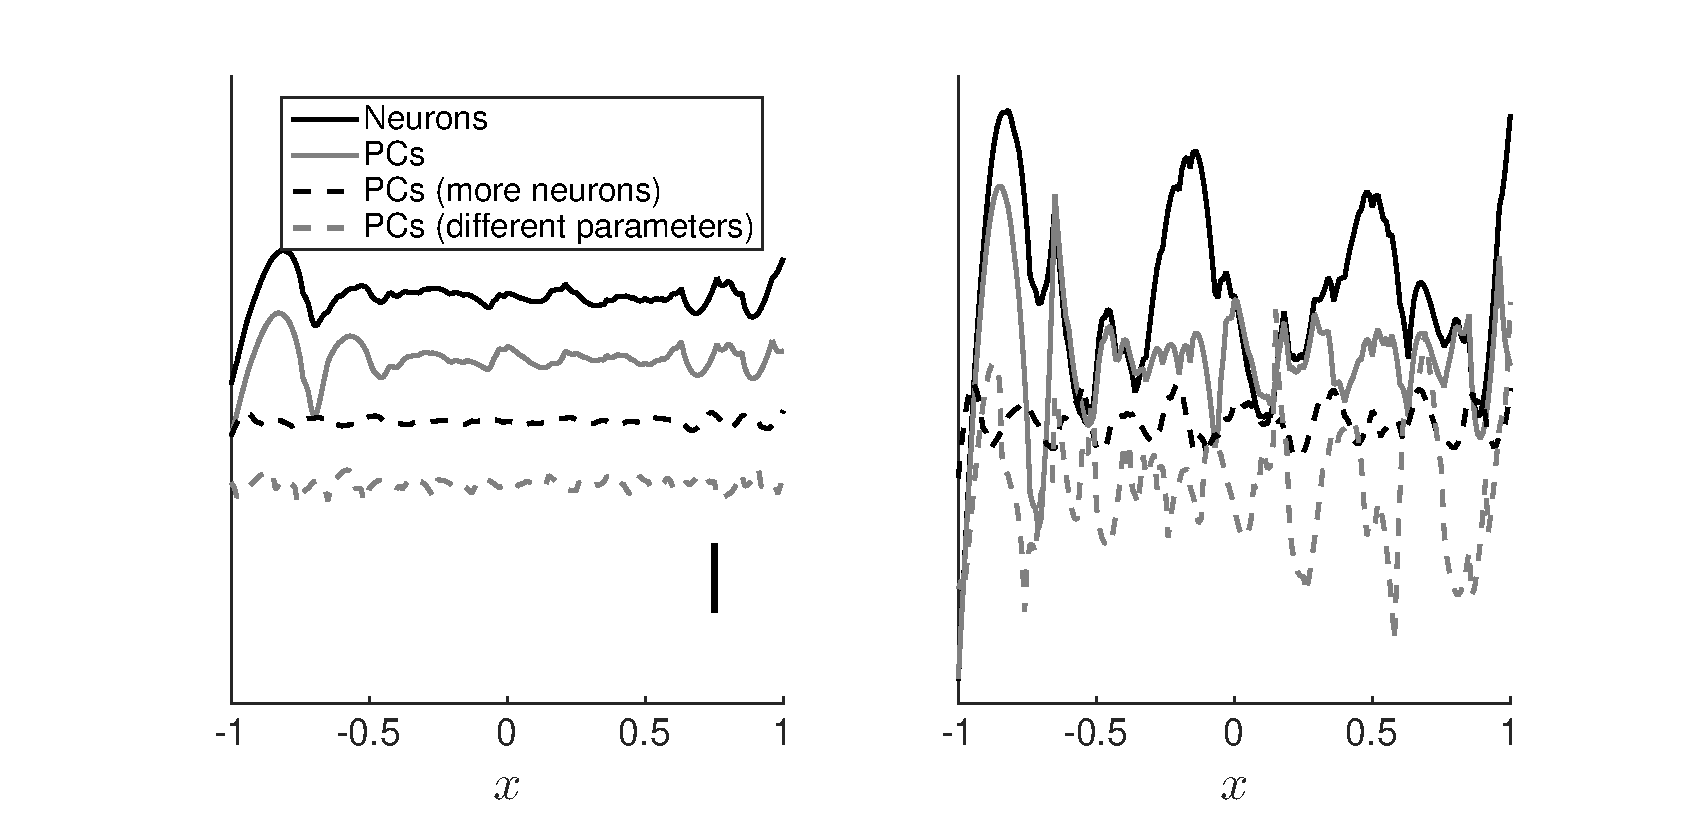
\includegraphics[scale=0.4]{shared-PCs.eps}
\caption{Comparison of bias error with different approximation schemes. The left panel shows bias errors in decoding the function $\sin(\pi x)$. The different error plots are offset vertically for clarity; the scale bar indicates an error magnitude of 0.1. The solid dark line shows decoding error from a population of 100 neurons (parameter set \#6). The solid light line below it shows decoding error from the first 15 principal components of the same population. The dark dashed line shows decoding error from the first 15 principal components of a larger population (500 neurons) with the same parameter distribution. The principal components of the larger population are smoother, and this error function has lower high-frequency content. Finally, the light dashed line shows decoding error from the first 15 principal components of a 100-neuron population with different parameters (parameter set \#1). The right panel shows analogous errors for decoding of $\sin(3 \pi x)$. As is typical, this higher-frequency function is not decoded as well, because it requires greater involvement of minor (noisier) principal components. } 
\label{fig:shared-pcs}
\end{figure}

\end{document}